This chapter can contain the following items:
\begin{itemize}
    \item Fundamental concepts and related terminologies (explain different terminologies used throughout the thesis)
    \item Related work
    \item Related technologies, algorithm, and parameters
\end{itemize}
\ cite command is use to cite any references stored in references.bib file as bibtex file.


\section{Figures}
There is a folder named figures; it is better to put all the figures in one folder. To find the figures more easily chapter wise folder of figures will be a great option
\subsection{One figure at a time}
The figure is shown below and can be referred such as \ref{label_figure}
\begin{figure}[h]
\centering
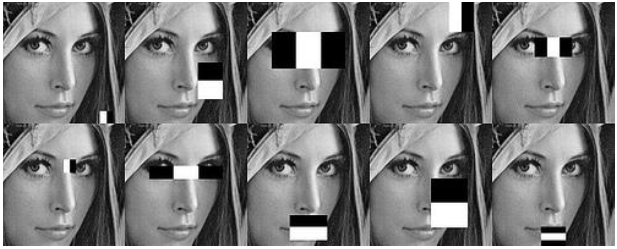
\includegraphics[width=90mm]{figures/Figure_chap2/haarf.PNG}
\caption{Features applied onto the face for matching facial characteristics}
\label{label_figure}
\end{figure}
The section \ref{subfig} shows how to put more than one pictures in one row.
\subsection{Subfigures}\label{subfig}
\begin{figure}[h]
\centering
\subfloat[Final 4 layers trainable.\label{cnf_mat_01}]{%
  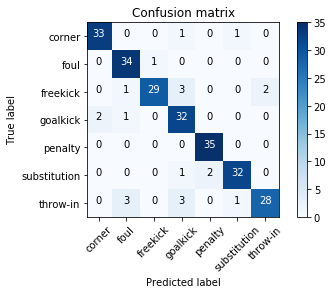
\includegraphics[width=0.5\textwidth]{figures/Figure_chap2/cnf_vgg16_4.png}%
}\hfil
\subfloat[Final 8 layers trainable.\label{cnf_mat_02}]{%
  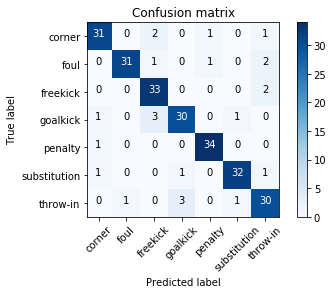
\includegraphics[width=0.5\textwidth]{figures/Figure_chap2/cnf_vgg16_8.png}%
}

\caption{VGG16 confusion matrix (a) final 4 layers trainable, (b) final 8 layers trainable.}
\label{fig_vgg16_cnf}
\end{figure}

\section{Table}
\subsection{soja table}
\section{Data collection of software modules}
\begin{table}[H]
\caption{Result of face, eye, and smile detection}
\label{swM1}
\begin{tabular}{|c|c|c|c|c|c|c|}
\hline
\multirow{2}{*}{\textbf{Participants}} & \multicolumn{2}{c|}{\textbf{Face Detection}} & \multicolumn{2}{c|}{\textbf{Eye Detection}} & \multicolumn{2}{c|}{\textbf{Smile Detection}} \\ \cline{2-7} 
                                       & \textbf{Total}      & \textbf{Detected}      & \textbf{Total}      & \textbf{Detected}     & \textbf{Total}       & \textbf{Detected}      \\ \hline
1                                      & 390                 & 385                    & 390                 & 375                   & 200                  & 180                    \\ \hline
2                                      & 425                 & 391                    & 425                 & 380                   & 223                  & 190                    \\ \hline
3                                      & 400                 & 375                    & 400                 & 370                   & 213                  & 183                    \\ \hline
4                                      & 401                 & 400                    & 401                 & 395                   & 200                  & 188                    \\ \hline
5                                      & 400                 & 380                    & 400                 & 377                   & 211                  & 187                    \\ \hline
6                                      & 430                 & 412                    & 430                 & 389                   & 209                  & 180                    \\ \hline
7                                      & 415                 & 400                    & 415                 & 379                   & 216                  & 170                    \\ \hline
8                                      & 401                 & 397                    & 401                 & 381                   & 219                  & 195                    \\ \hline
9                                      & 397                 & 393                    & 397                 & 379                   & 214                  & 187                    \\ \hline
10                                     & 396                 & 392                    & 396                 & 375                   & 207                  & 199                    \\ \hline
\textbf{mean}                          & 405.5               & 392.5                    & 405.5               & 380                   & 211.2                & 185.9                  \\ \hline
\textbf{variance}                      &                     & 114.9444444            &                     & 52                    &                      & 67.65555556            \\ \hline
\textbf{STDEV}                         &                     & 10.72121469            &                     & 7.211102551           &                      & 8.225299724            \\ \hline
\textbf{$\sqrt{N}$}                    & \multicolumn{6}{c|}{3.16227766}                                                                                                            \\ \hline
\textbf{$SEM$}           &                     & 3.390345771            &                     & 2.28035085            &                      & 2.601068157            \\ \hline
\end{tabular}
\end{table}
\subsection{kemon kemon table}

\begin{table}[H]
\centering
\caption{Quantitative data collection of three responsive behavior of the robot}
\label{aware1}
\rotatebox{90}{
\begin{tabular}{|c|c|c|c|c|c|c|c|c|c|c|}
\hline
\multirow{2}{*}{\textbf{\begin{tabular}[c]{@{}c@{}}\# of \\ Exp\end{tabular}}} & \multicolumn{5}{c|}{\textbf{Human Initiative Case}}                   & \multicolumn{5}{c|}{\textbf{Robot Initiative Case}}                  \\ \cline{2-11} 
                                                                               & \multicolumn{3}{c|}{\textbf{Methods}}   & \textbf{}    & \textbf{}    & \multicolumn{3}{c|}{\textbf{Methods}}   & \textbf{}    & \textbf{}    \\ \hline
\textbf{}                                                                      & \textbf{M1} & \textbf{M2} & \textbf{M3} & \textbf{Age} & \textbf{F/M} & \textbf{M1} & \textbf{M2} & \textbf{M3} & \textbf{Age} & \textbf{F/M} \\ \hline
1                                                                              & 1           & 1           & 1           & 22           & F            & 1           & 1           & 1           & 26           & F            \\ \hline
2                                                                              & 1           & 1           & 1           & 21           & F            & 1           & 1           & 1           & 24           & M            \\ \hline
3                                                                              & 1           & 1           & 1           & 21           & F            & 1           & 1           & 0           & 24           & F            \\ \hline
4                                                                              & 1           & 1           & 0           & 20           & F            & 1           & 1           & 0           & 27           & F            \\ \hline
5                                                                              & 1           & 1           & 0           & 22           & F            & 0           & 1           & 0           & 27           & M            \\ \hline
6                                                                              & 1           & 1           & 0           & 21           & F            & 0           & 1           & 0           & 27           & M            \\ \hline
7                                                                              & 1           & 1           & 0           & 21           & F            & 0           & 1           & 0           & 25           & F            \\ \hline
8                                                                              & 1           & 1           & 0           & 21           & F            & 0           & 0           & 0           & 22           & M            \\ \hline
9                                                                              & 1           & 1           & 0           & 21           & F            & 0           & 1           & 0           & 21           & F            \\ \hline
10                                                                             & 0           & 1           & 0           & 21           & F            & 1           & 1           & 1           & 21           & F            \\ \hline
11                                                                             & 0           & 1           & 0           & 21           & M            & 0           & 1           & 0           & 21           & F            \\ \hline
12                                                                             & 0           & 1           & 0           & 21           & M            & 1           & 1           & 1           & 20           & F            \\ \hline
13                                                                             & 0           & 1           & 0           & 21           & M            & 0           & 1           & 0           & 20           & M            \\ \hline
14                                                                             & 0           & 1           & 0           & 21           & M            & 1           & 0           & 0           & 20           & M            \\ \hline
15                                                                             & 0           & 1           & 0           & 21           & M            & 0           & 1           & 0           & 21           & M            \\ \hline
16                                                                             & 0           & 1           & 0           & 22           & M            & 0           & 1           & 0           & 21           & M            \\ \hline
Total                                                                          & 9           & 16          & 3           & 338          & M            & 7           & 14          & 4           & 367          &              \\ \hline
Mean                                                                           & 0.56        & 1           & 0.19        & 21.13        &              & 0.44        & 0.88        & 0.25        & 22.94        &              \\ \hline
STD                                                                            & 0.49        & 0           & 0.39        & 0.48         &              & 0.49        & 0.33        & 0.43        & 2.63         &              \\ \hline
\end{tabular}}
\end{table}
Table~\ref{aware1} example of normal table with multi row multi column with 90\degree rotation
\subsection{Sub table}\label{subtable}
\begin{table}[!htb]
    \caption{Global caption}
    \begin{subtable}{.5\linewidth}
      \centering
        \caption{}
        \begin{tabular}{ll}
            1 & 2
        \end{tabular}
    \end{subtable}%
    \begin{subtable}{.5\linewidth}
      \centering
        \caption{}
        \begin{tabular}{ll}
            3 & 4
        \end{tabular}
    \end{subtable} 
\end{table}